\section{Results}
As expected bidirectional path tracing yielded better results with less samples per pixel (SPP) in the same or even less time than normal (shooting rays from the view point) path tracing. We set the number of light ray (LR) bounces to two, since more bounces only slightly improved the resulting image quality while drastically increasing the rendering time. In \ref{fig:comparison_1_npt} and \ref{fig:comparison_1_bpt} we used a simple scene. Normal path tracing \ref{fig:comparison_1_npt} took 34 seconds while bidirectional path tracing \ref{fig:comparison_1_bpt} took only 31 seconds, while rendering the back wall less grainy. In \ref{fig:comparison_2_npt} and \ref{fig:comparison_2_bpt} we used a scene with a translucent sphere. Again, bidirectional path tracing \ref{fig:comparison_2_bpt} took less time using less SPP then normal path tracing \ref{fig:comparison_2_npt}.

\begin{figure}[htbp]
  \centering
     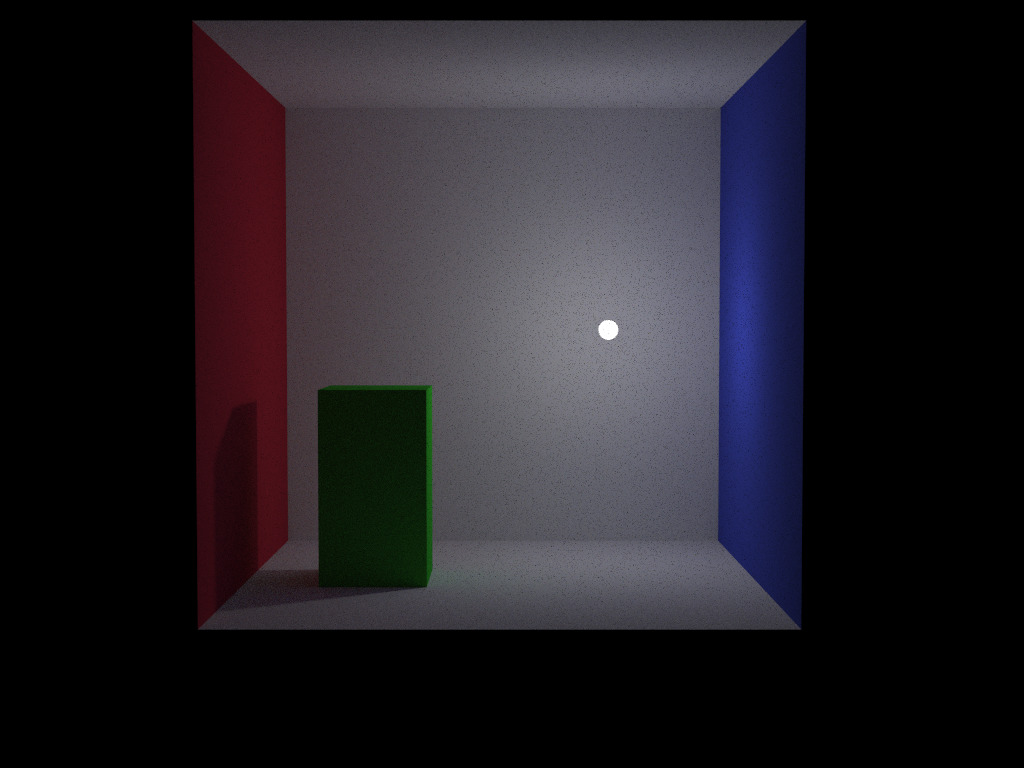
\includegraphics[width=\textwidth]{pics/1_normal_pt_16spp_34s.jpg}
  \caption{Normal path tracing with 16 SPP took 34s}
  \label{fig:comparison_1_npt}
\end{figure}

\begin{figure}[htbp]
  \centering
     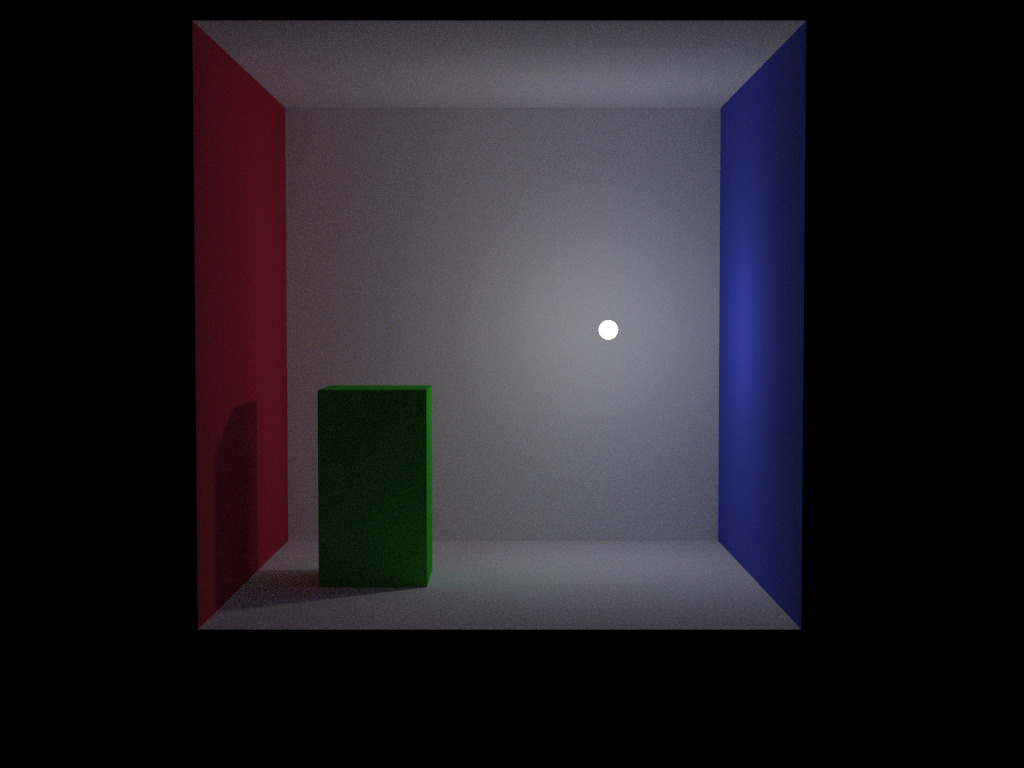
\includegraphics[width=\textwidth]{pics/1_bi_dir_pt_8spp_2lrb_31s.jpg}
  \caption{Bidirectional path tracing with 8 SPP and 2 LR bounces took 31s}
  \label{fig:comparison_1_bpt}
\end{figure}

\begin{figure}[htbp]
  \centering
     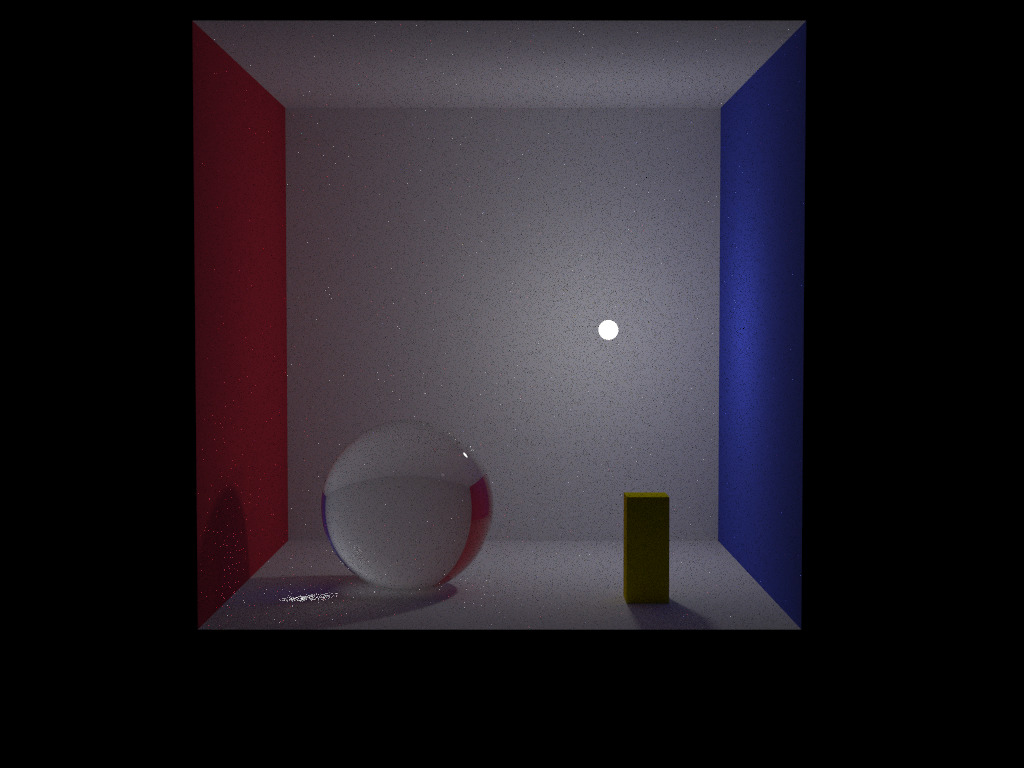
\includegraphics[width=\textwidth]{pics/2_normal_pt_32spp_75s.jpg}
  \caption{Normal path tracing with 32 SPP took 75s}
  \label{fig:comparison_2_npt}
\end{figure}

\begin{figure}[htbp]
  \centering
     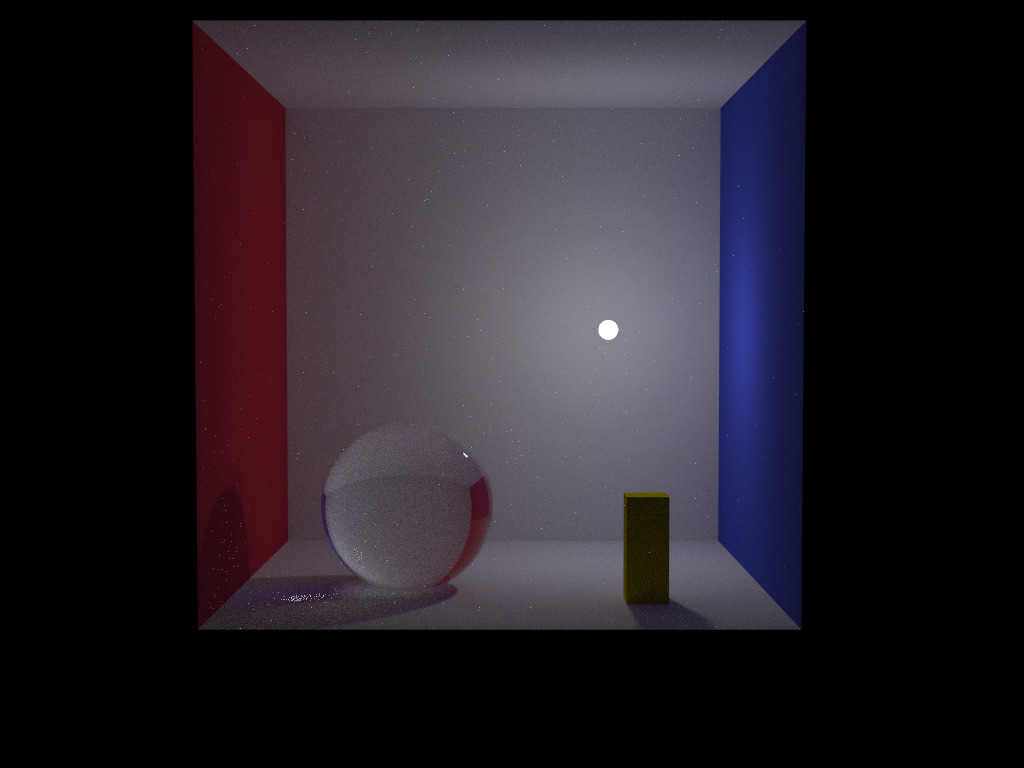
\includegraphics[width=\textwidth]{pics/2_bi_dir_pt_16spp_2lrb_58s.jpg}
  \caption{Bidirectional path tracing with 16 SPP and 2 LR bounces took 58s}
  \label{fig:comparison_2_bpt}
\end{figure}